% Four finite views of the same fair-coin experiment. Each rust segment
% has relative length 2^{-n}; this is not simulated data.
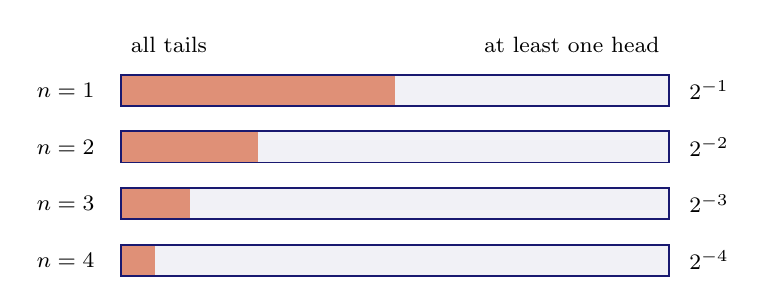
\begin{tikzpicture}[x=0.87cm,y=0.72cm,line cap=round]
  \foreach \k/\yy/\ww in {1/3/4,2/2/2,3/1/1,4/0/0.5}{
    \fill[MidnightBlue!6] (2,\yy) rectangle (10,{\yy+0.55});
    \fill[BrickRed!42] (2,\yy) rectangle ({2+\ww},{\yy+0.55});
    \draw[MidnightBlue,line width=0.65pt] (2,\yy) rectangle (10,{\yy+0.55});
    \node[font=\footnotesize,anchor=east] at (1.75,{\yy+0.275}) {$n=\k$};
    \node[font=\footnotesize,anchor=west] at (10.15,{\yy+0.275}) {$2^{-\k}$};
  }
  \node[font=\footnotesize,anchor=west] at (2,4.08) {all tails};
  \node[font=\footnotesize,anchor=east] at (10,4.08) {at least one head};
\end{tikzpicture}
